\documentclass[tikz,multi,border=10pt]{standalone}
\usetikzlibrary{shadows,arrows.meta,positioning,backgrounds,fit,chains,scopes}

% Define block styles
\tikzset{%
  materia/.style={draw, fill=blue!20, text width=6.0em, text centered, minimum height=1.5em,drop shadow},
  etape/.style={materia, text width=8em, minimum width=10em, minimum height=3em, rounded corners, drop shadow},
  linepart/.style={draw, thick, color=black!50, -LaTeX, dashed},
  line/.style={draw, thick, color=black!50, -LaTeX},
  ur/.style={draw, text centered, minimum height=0.01em},
  back group/.style={fill=yellow!20,rounded corners, draw=black!50, dashed, inner xsep=15pt, inner ysep=10pt},
}

\newcommand{\transreceptor}[3]{%
  \path [linepart] (#1.east) -- node [above] {\scriptsize #2} (#3);}

\begin{document}
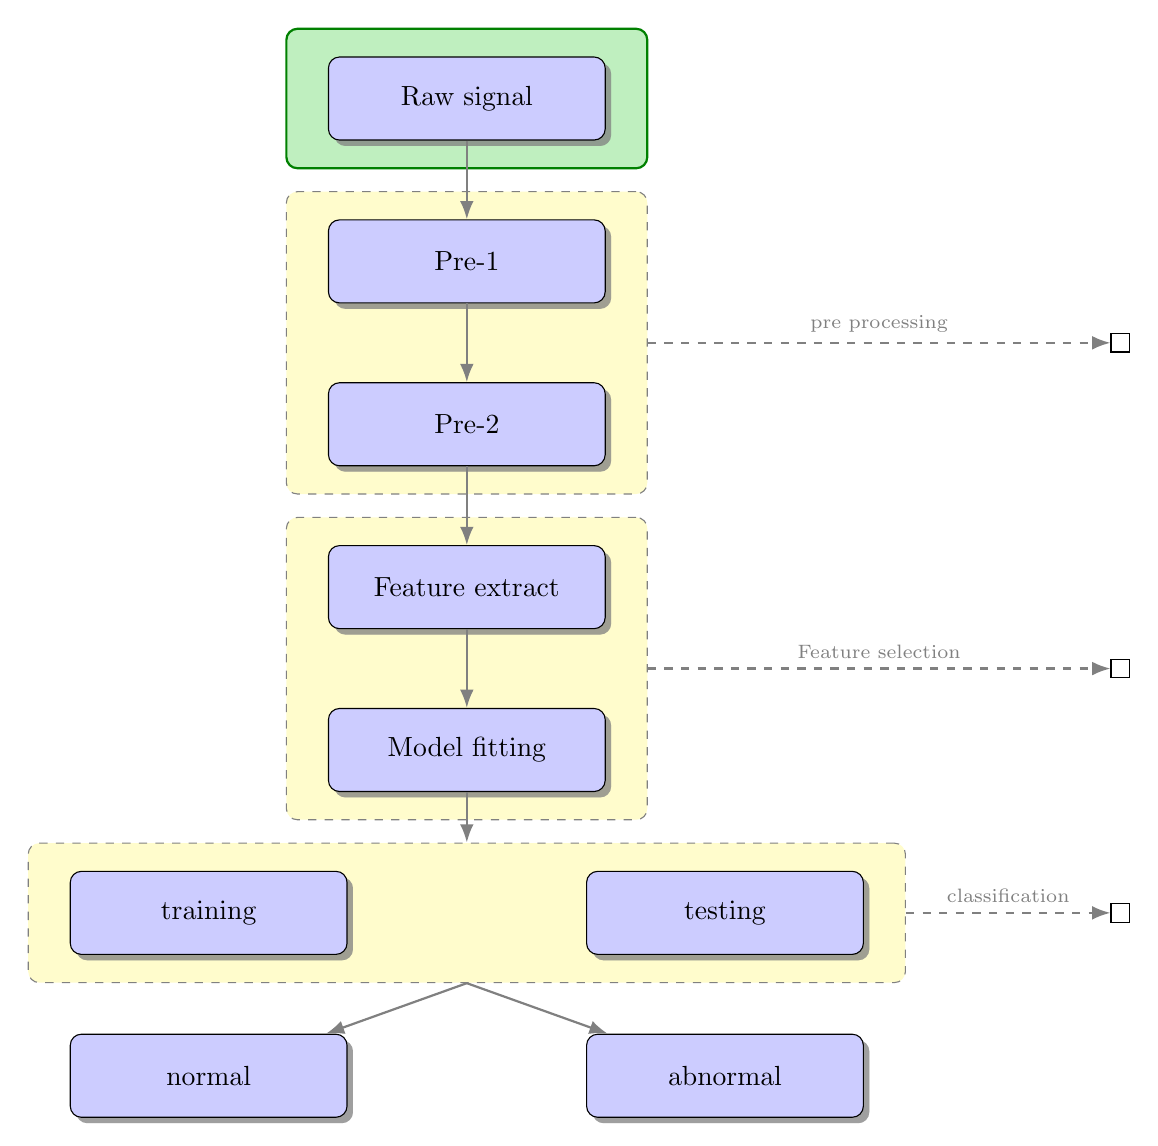
\begin{tikzpicture}
  [
    start chain=p going below,
    every on chain/.append style={etape},
    every join/.append style={line},
    node distance=1 and -.25,
  ]
  {
    \node [on chain, join] {Raw signal};
    \node [on chain, join] {Pre-1};
    \node [on chain, join] {Pre-2};
    \node [on chain, join] {Feature extract};
    \node [on chain, join] {Model fitting};
    {[start branch=r going below right]
      \node [on chain] {testing};
    }
    {[start branch=l going below left]
      \node [on chain] {training};
    }
    {[continue branch=r going below]
      \node [on chain] {abnormal};
    }
    {[continue branch=l going below]
      \node [on chain] {normal};
    }
  }

  \begin{scope}[on background layer]
    \node (bk1) [back group] [fit=(p-2) (p-3)] {};
    \node (bk2) [back group] [fit=(p-4) (p-5)] {};
    \node (bk3) [back group] [fit=(p/r-2) (p/l-2)] {};
    \node [draw, thick, green!50!black, fill=green!75!black!25, rounded corners, fit=(p-1), inner xsep=15pt, inner ysep=10pt] {};
  \end{scope}

  \path [line] (p-5.south) --  (bk3.north);
  \path [line] (bk3.south) --  (p/l-3);
  \path [line] (bk3.south) --  (p/r-3);
  \path (bk1.east)+(+6.0,0) node (ur1)[ur] {};
  \node (ur2)[ur] at (bk2.east -| ur1) {};
  \node (ur3)[ur] at (bk3.east -| ur1) {};
  \transreceptor{bk1}{pre processing}{ur1};
  \transreceptor{bk2}{Feature selection}{ur2};
  \transreceptor{bk3}{classification}{ur3};
\end{tikzpicture}
\end{document}